\section{Aufgabe 1}
\begin{center}
\begin{minipage}{\linewidth}
\centering
\makebox[0cm]{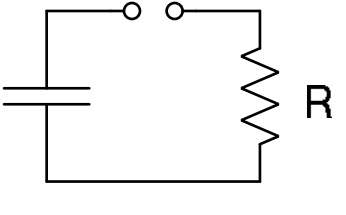
\includegraphics[scale=0.5]{sb1}}
\captionof{figure}{Schaltplan Aufgabe 1}%
\label{schaltplan_nr1}
\end{minipage}
\end{center}

Für diese Aufgabe haben wir einen Kondensator mit einem Widerstand in Reihe geschalten (siehe Abbildung 1.1). Mit einem Frequenzgenerator legten wir eine Spannung an und mit Hilfe eines Oszilloskops veränderten wir die Frequenz, bis beide Sinuskurven die gleiche Spannung hatten. 
Damit die Teilspannung an der Spule und am Kondensator übereinstimmen muss folgendes gelten:
\begin{equation}
U_C = U_R 	\Rightarrow	 U_{ges} = U_C + U_R
\end{equation}
Mit einem Spannungsmessgerät (Fluke 175) haben wir die Spannung zwischen dem Widerstand und dem Kondensator gemessen. Dabei betrug der Spannungsunterschied:
\begin{equation}
\notag
\Delta U=0,023 V
\end{equation}

Die Frequenz betrug dabei konstant:

\begin{equation}\notag
f_{char} = (160,45\pm 0,1) Hz
\end{equation}

Die verwendeten Bauteile des R-C-Kreises wurden separat noch einmal nachgemessen, dabei ergab sich für den Widerstand einen Wert von:
\begin{equation}\notag
R = (0.990 \pm 0.012)k\Omega
\end{equation}

und die Kapazität des Kondensators:
\begin{equation}\notag
C = (1.001 \pm 0.013)\mu F
\end{equation}

Die Fehler errechnen sich aus $\pm (1.0\% +3dgt)$.

\subsection{Berechnung der Frequenz}
Nun können wir über folgende Formel den theoretischen Wert der Frequenz f berechnen:
\begin{equation}\notag
f_{theo}=\frac{1}{2\pi RC}= (160.6 \pm 2.0)Hz
\end{equation}

Den Fehler bestimmen wir über die Gauß'sche Fehlerfortpflanzung:
\begin{equation}\notag
\Delta f_{theo}=\sqrt{\left(\frac{\partial f_{theo}}{\partial R}\cdot \Delta R\right)^2+\left(\frac{\partial f_{theo}}{\partial C}\cdot \Delta C\right)^2}
\end{equation}

\subsection{Phasenverschiebung}
Für die Phasenverschiebung haben wir bei einer Frequenz von f = 160,30 HZ am Oszilloskop ein \(\Delta\)t = 0,8ms abgelesen. Dafür ergibt sich für \(\phi\) einen Wert für:
\begin{equation}
\notag
\phi = 2\pi f \Delta t = (0,806 \pm 0,009)^\circ = (0,257\pm 0,003)\pi
\end{equation}

Somit ergibt sich wie erwartet \(\frac{\pi}{4}\) für die Phasenverschiebung.
Um nun noch die Phasenverschiebung auszurechnen, benutzten wir:
\begin{equation}\notag
\phi_{theo}=arctan\left(\frac{1}{\omega RC}\right)=\left(0,7854 \pm 0.0065\right)^\circ =(0,250\pm 0,003)\pi
\end{equation}

Den Fehler bekommen wir aus:
\begin{equation}\notag
\Delta \phi_{theo}=\sqrt{\left(\frac{\partial \phi_{theo}}{\partial f_{theo}}\cdot \Delta f_{theo}\right)^2+\left(\frac{\partial \phi_{theo}}{\partial C}\cdot \Delta C\right)^2+\left(\frac{\partial \phi_{theo}}{\partial R}\cdot \Delta R\right)^2}
\end{equation}

\subsection*{Fazit}
Den Wert für die charakteristische Frequenz konnten wir relativ schnell finden, nachdem wir festgestellt hatten, dass ein Messgerät einen Wackelkontakt hatte und bis dahin nur seltsame Werte geliefert wurden.\\
Der theoretische und der gemessene Wert der charakteristische Frequenz sind gleich, nur dass der Fehler des theoretischen Werts aufgrund der Bauteile doch relativ groß ist. Die Phasenverschiebung ist auch ziemlich klein.